\section{Overview}\label{sec:overview}

\begin{figure}
  \centering
  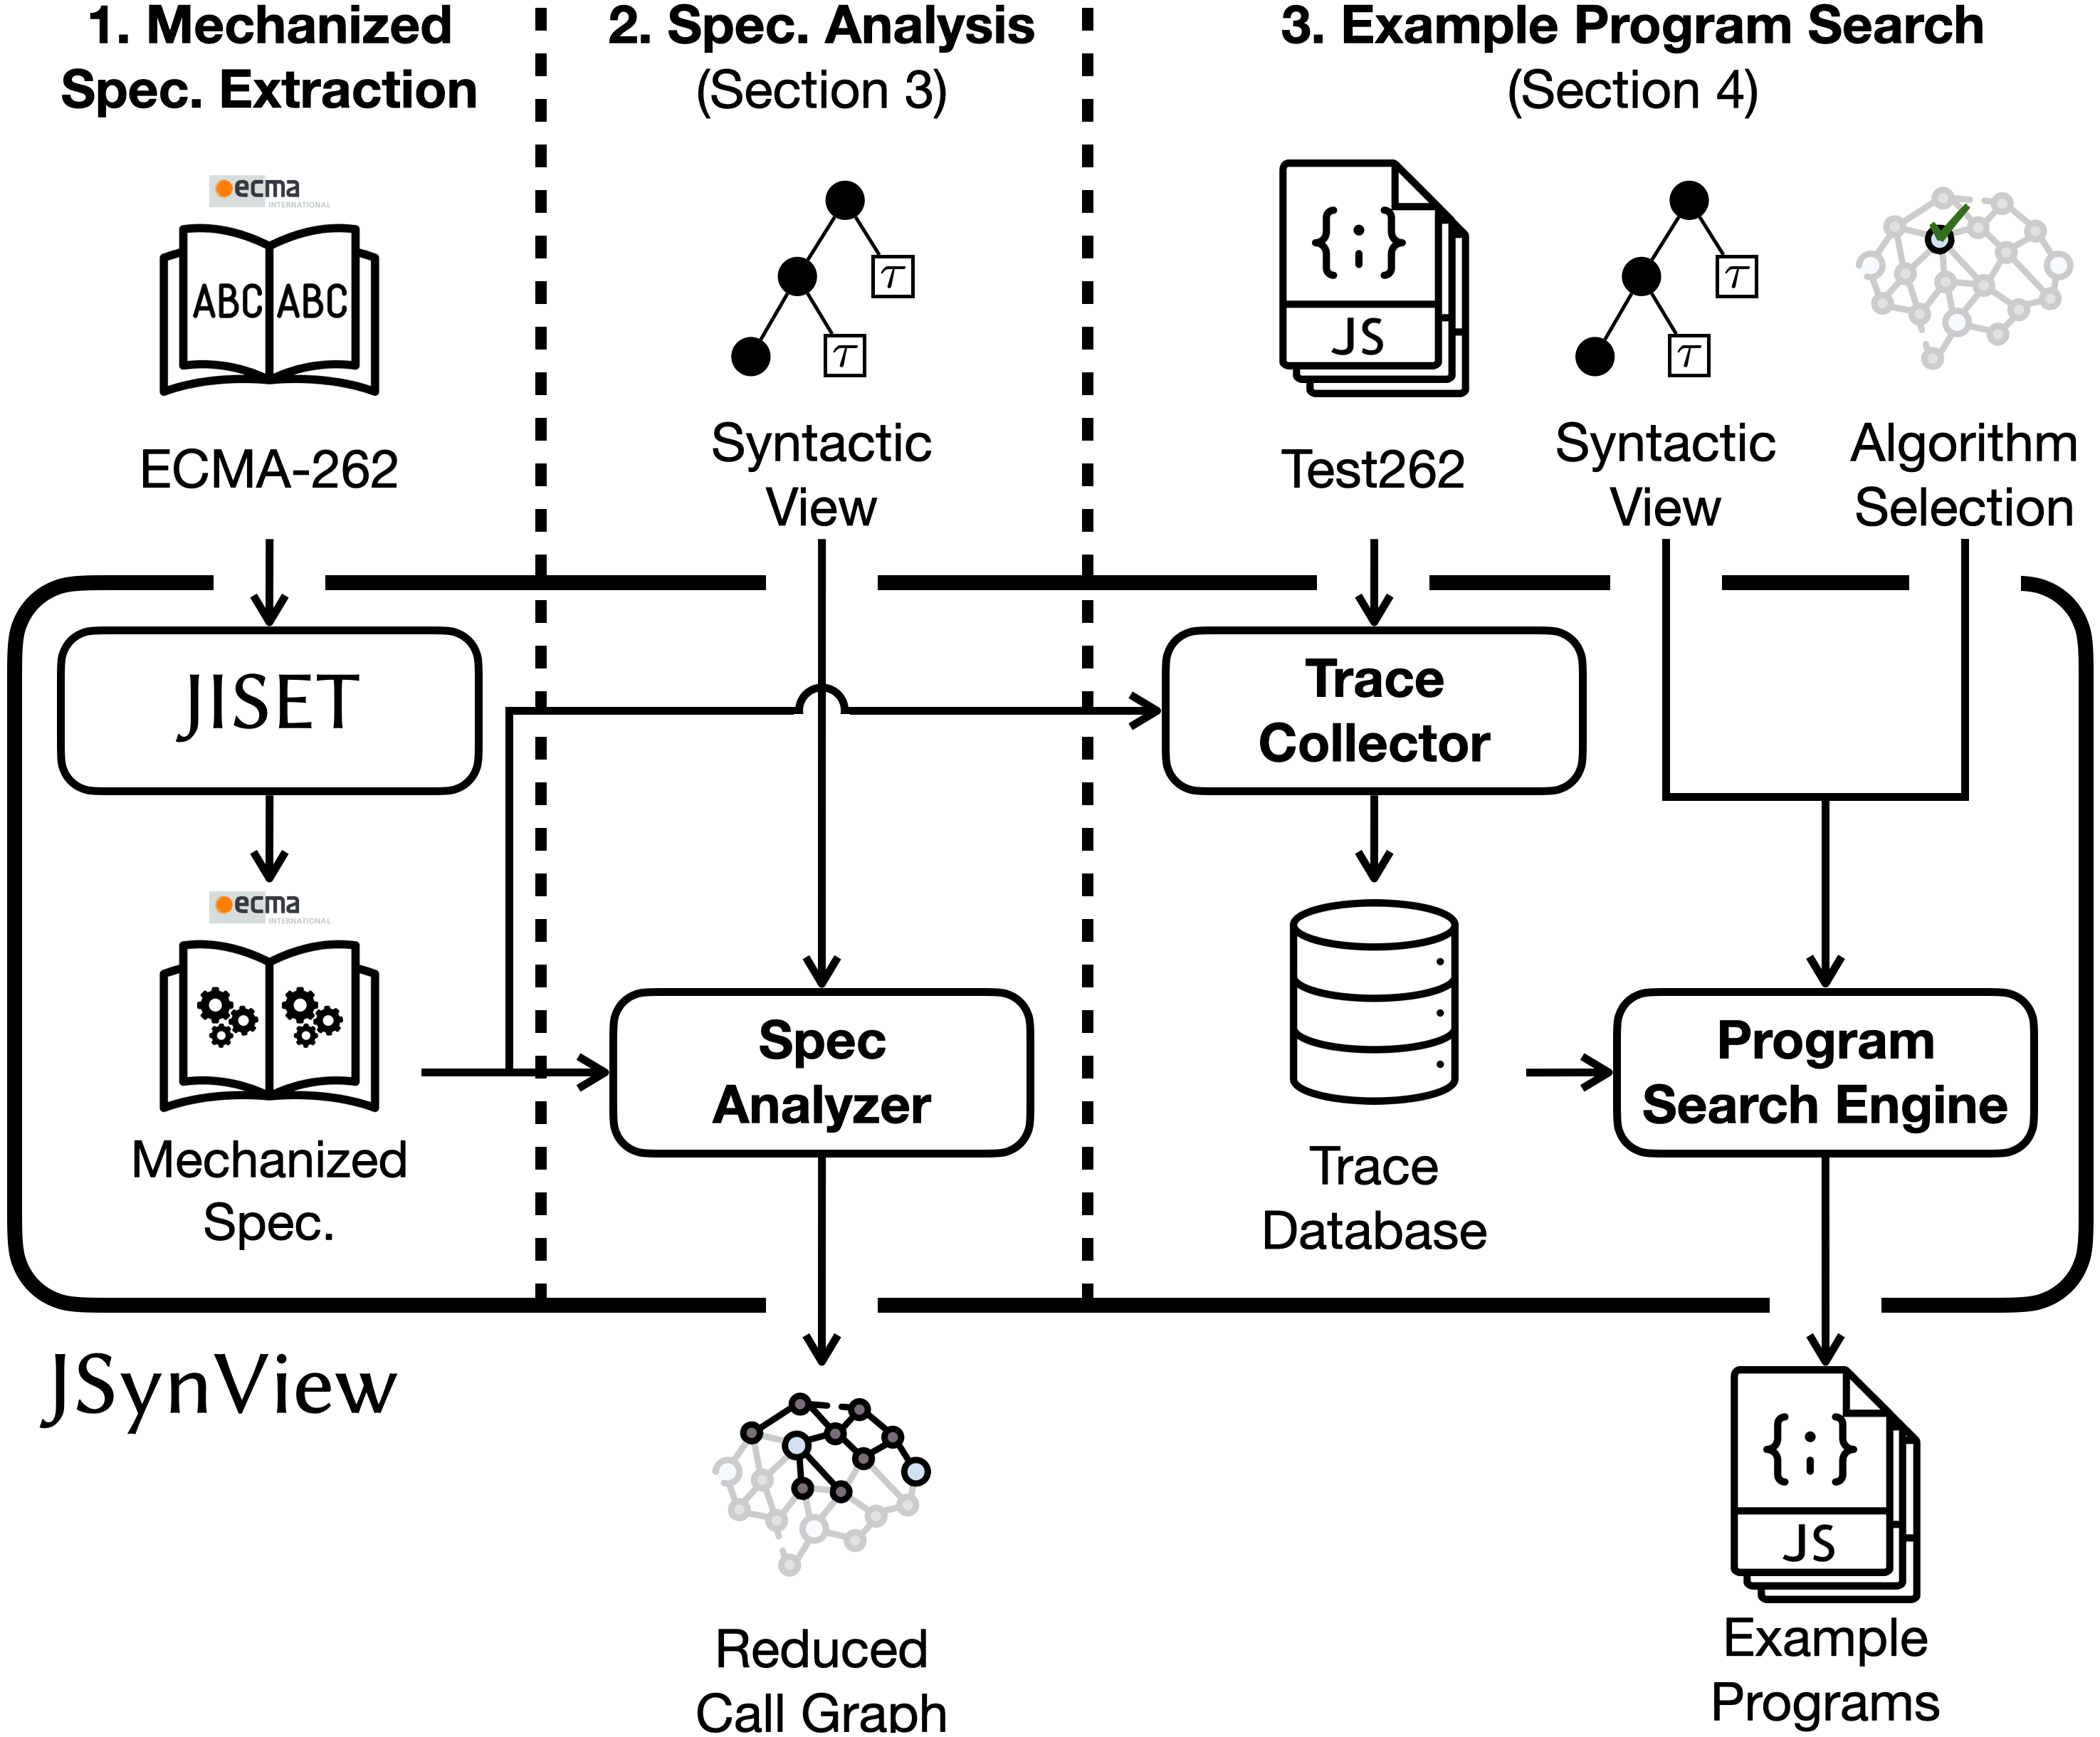
\includegraphics[width=\columnwidth]{img/overall.png}
  \caption{Overall structure of $\tool$}
  \vspace*{-1em}
  \label{fig:overall}.
\end{figure}

This section explains the overall structure of $\tool$ depicted in
Figure~\ref{fig:overall} with simple examples.  It consists of three phases: 1)
\textit{mechanized specification extraction}, 2) \textit{behavior inference} and
3) \textit{example program search}.

\subsection{Mechanized Specification Extraction}\label{sec:extract-spec}

As explained in Section~\ref{sec:intro}, ECMA-262 is the standard JavaScript
language specification defining the semantics using abstract algorithms
consisting of structured steps written in English.  Thus, it is difficult to
handle it in an automatic or mechanical way.  However, fortunately,
\citet{jiset} introduced $\jiset$, which extracts a mechanized specification
from any given version of ECMA-262.  They defined $\ires$, an intermediate
representation for ECMAScript, to compile algorithms and their steps to $\ires$
functions and instructions, respectively.  Therefore, the extracted mechanized
specification form a given ECMA-262 is an $\ires$ program consisting of
functions corresponding to abstract algorithms in the language specification.
In this paper, we use its newer platform $\esmeta$~\cite{esmeta} an
\underline{E}CMAScript \underline{S}pecification \underline{M}etalnaguage,
because it is more actively mainitained rather than $\jiset$.


\subsection{Behavior Inference}\label{sec:reduce-spec}

\begin{figure}
  \centering
  \begin{subfigure}[t]{\columnwidth}
    \centering
    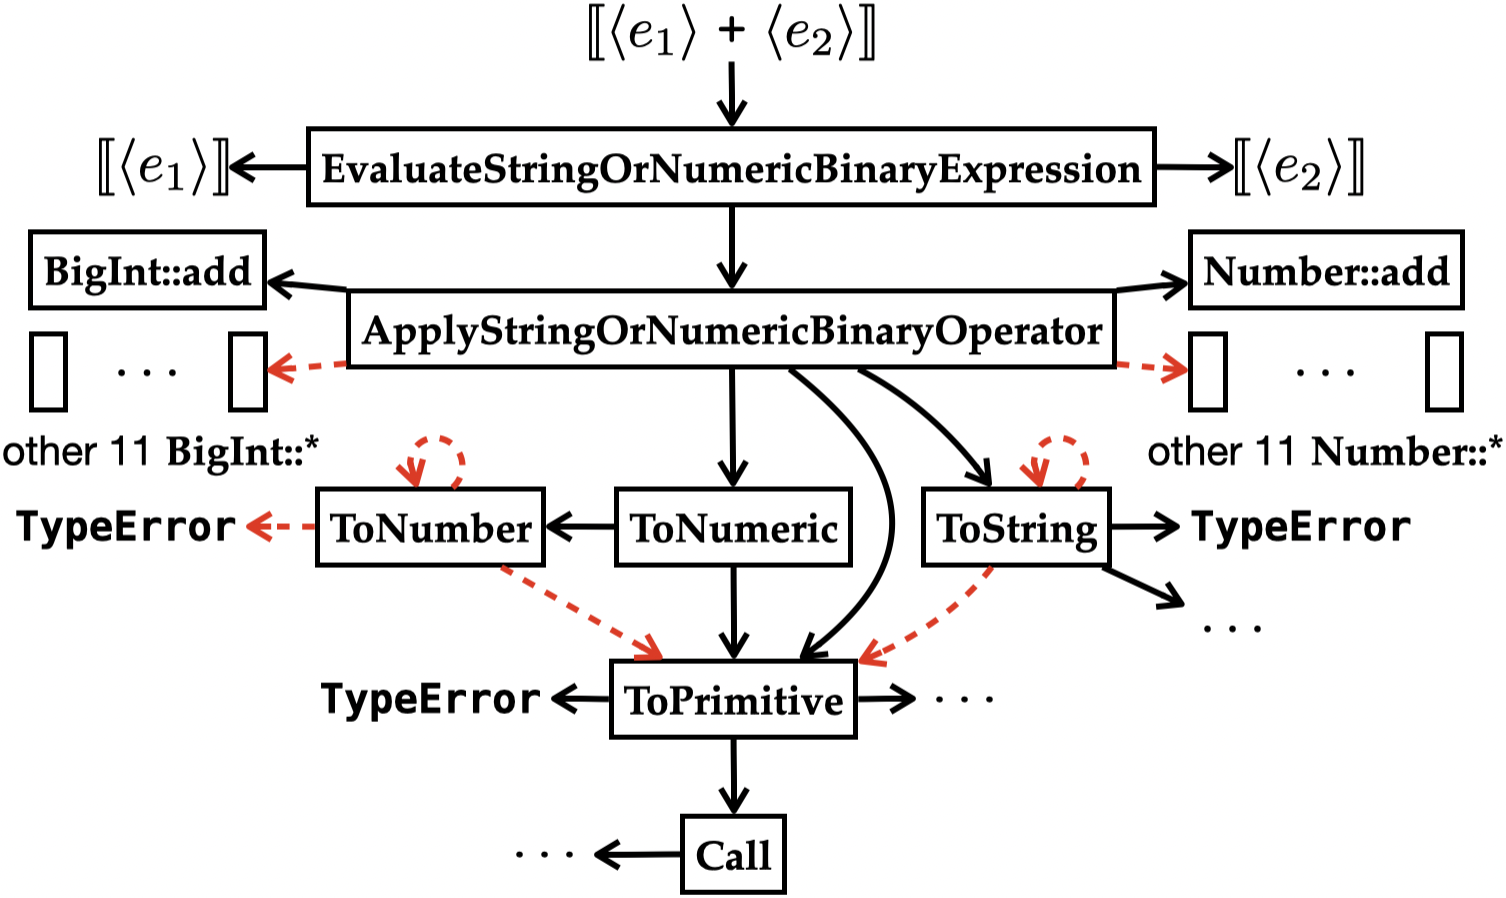
\includegraphics[width=\textwidth]{img/add-basic.png}
    \caption{Reduced call graph with $\svhole{\expr_1} \; \code{+} \;
    \svhole{\expr_2}$}
  \end{subfigure}
  \begin{subfigure}[t]{\columnwidth}
    \centering
    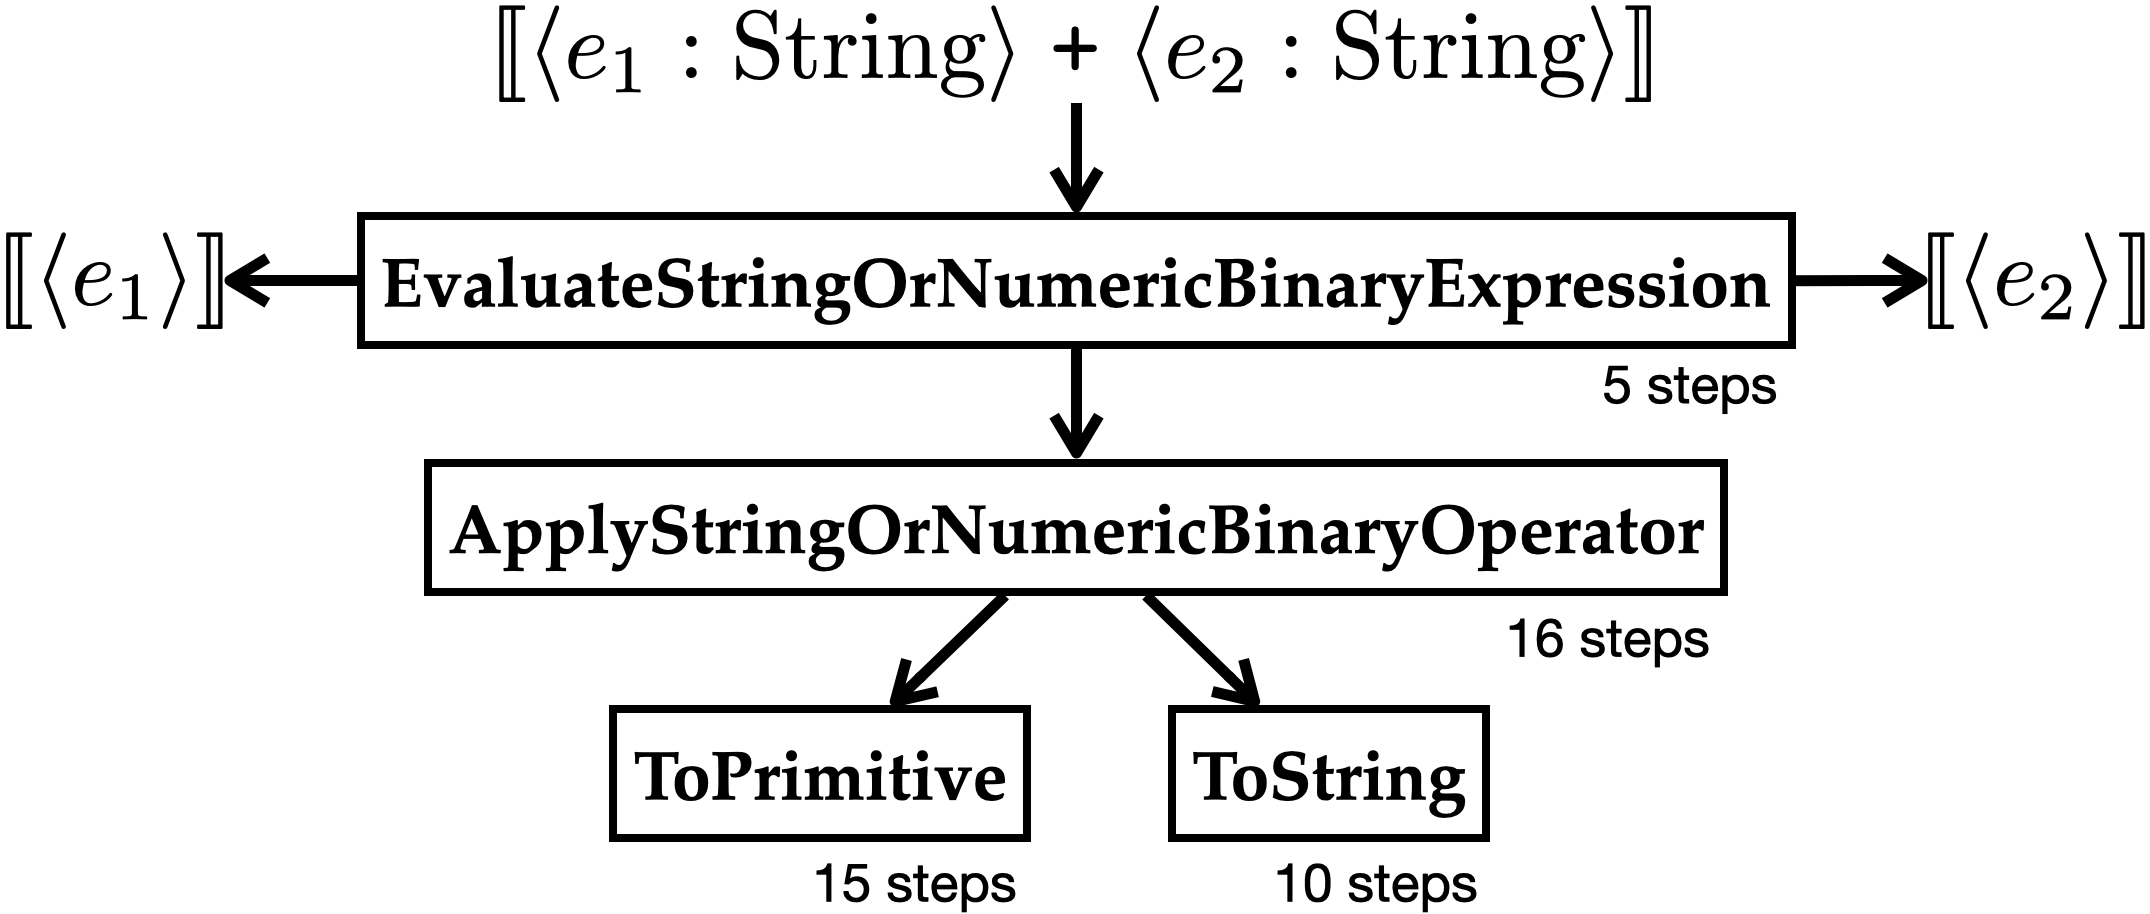
\includegraphics[width=.8\textwidth]{img/add-str.png}
    \caption{Reduced call graph with $\svhole{\expr_1: \text{String}} \;
    \code{+} \; \svhole{\expr_2: \text{String}}$}
  \end{subfigure}
  \caption{A call graph of the JavaScript language specification reduced with
    two different syntactic views}
  \vspace*{-1em}
  \label{fig:add-graph}.
\end{figure}

After extracting the mechanized specification, $\tool$ automatically infers
\textit{possible behaviors} of language features using the reachability analysis
in ECMA-262.  Users can select the target language feature they want to
understand by defining a \textit{syntactic view}, which is an extension of a
JavaScript AST with abstract nodes and optional type bounds.  It restricts
syntax and expected types of evaluation results of JavaScript programs.  For
example, assume that we want to understand the detailed semantics of JavaScript
addition operator (\code{+}) by referring to the latest ECMA-262 (ES12, 2021).
Then, we can utilize a syntactic view $\svhole{\expr_1} \; \code{+} \;
\svhole{\expr_2}$ where $\svhole{\expr_1}$ and $\svhole{\expr_2}$ denote
arbitrary expressions wihtout any type bounds.  For this syntactic view, the
reachability analyzer first finds \esalg{Evaluation} algorithm of the addition
operator shown in Figure~\ref{fig:add-eval-algo} as the initial point of the
analysis.  Then, it builds reduced call graphs consisting of the algorithms only
reachable from the initial algorithm.

Figure~\ref{fig:add-graph}(a) depicts the a call graph built by following all
algorithms starting from the \esalg{Evaluation} algorithm.  In this graph, a
node denotes 1) an abstract algorithm (box), 2) evaluation of syntactic view
($\sem{-}$), or 3) an exception (bold without box), and an arrow denotes a call
edge.  Among them, specific algorithms represent possible behaviors of the
addition operator.  For instance, the \esalg{Call} algorithm is used to call the
\eswrd{[[Call]]} internal method of a JavaScript function object.  It means that
a JavaScript function might be invoked during the evaluation of the addition
operator.  Besides, the addition operator might throw a \esval{TypeError}
exception because it is reachable from the \esalg{Evaluation} algorithm through
\esalg{ToNumber}, \esalg{ToString}, and \esalg{ToPrimitive}.

However, this call graph contains invalid edges for the evaluation of the
addition operator, and red dotted arrows in Figure~\ref{fig:add-basic} denote
such cases.  For example, \esalg{ApplyStringOrNumericBinaryOperator} only
invokes two different numeric methods \esalg{BigInt::add} and
\esalg{Number::add} for the evaluation of the addition oeprator.  Other 22
numeric methods, such as \esalg{BigInt::subtract} and \esalg{Number::divide},
are unreachable.  Moreover, \esval{TypeError} is throwable only in
\esalg{ToPrimitive} and \esalg{ToString} but not in \esalg{ToNumber} for the
addition operator.

Beyond basic syntactic restriction, we can give a more restriction to a
syntactic view with 1) type bounds or 2) combination with other language
features.  For instance, assume that we want to understand the addition between
string values.  Then, the syntactic view $\svhole{\expr_1: \text{String}} \;
\code{+} \; \svhole{\expr_2: \text{String}}$ represents such cases, and
Figure~\ref{fig:add-graph}(b) depicts the reduced call graph with this syntactic
view, and gives more information of the addition oeprator.  First, the addition
between string values never throws exceptions because there is no reachable
exceptions in this call graph.  Second, the string addition never invoke other
JavaScript functions because the \esalg{Call} algorithm is no longer reachable
from the \esalg{Evaluation} algorithm.  We can even restrict the expected
results of the abstract nodes using exceptions as type bounds: $\svhole{\expr_1:
\bot} \; \code{+} \; \svhole{\expr_2: \bot}$, where $\bot$ denotes an exception:
\begin{figure}[H]
  \centering
  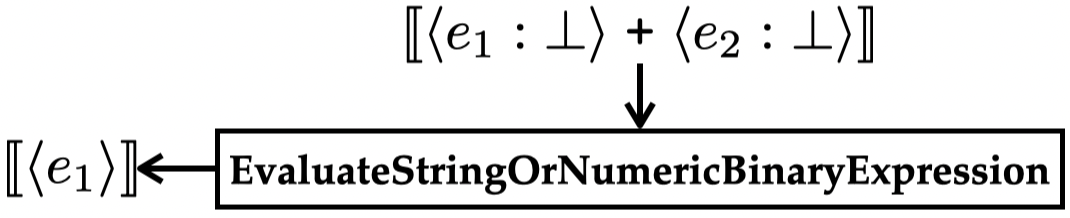
\includegraphics[width=.7\columnwidth]{img/add-exc.png}
\end{figure} \noindent
In this case, we notice that only left operand is evaluated when both left and
right operand throw exceptions.  Besides, we can combine different language
features in syntactic views.  For example, a syntactic view $\svhole{\expr_1:
\text{Number}} \; \code{+} \; \svhole{\expr_2: \text{Number}} \; \code{*} \;
\svhole{\expr_3: \text{Number}}$ represents the combination of numeric addition
and multiplication.





\subsection{Example Program Search}\label{sec:reduce-spec}

While the reachability analysis with a given syntactic view provides possible
behaviors of the corresponding language feature, it is another challenging
problem to find concrete example programs that trigger a specific behavior.  For
example,


\begin{itemize}
  \item In Figure~\ref{fig:add-basic}
    \begin{itemize}
      \item TypeError in ToString:
        \code{test/language/expressions/addition/symbol-to-string.js}
      \item Call:
        \code{test/language/expressions/addition/S11.6.1\_A2.2\_T1.js}
    \end{itemize}
\end{itemize}
